\documentclass{../industrial-development}
\graphicspath{{09-profiling-and-static-analysis/}}

\title{Инструменты профилирования и~статического анализа кода в~промышленной разработке}
\author{Мартынов Андрей Олегович, ИВТ--21 МО}
\date{}

\begin{document}

\begin{frame}
  \titlepage
\end{frame}

\begin{frame}{План лекции}
	\tableofcontents
\end{frame}

\section{Назначение процедуры профилирования кода}

\begin{frame} \frametitle{Назначение процедуры профилирования кода}
  \begin{block}{}
    \alert{Процедура профилирования кода} помогает разработчику найти проблемы с производительностью и даёт возможность отследить:
	\end{block}
  
  \begin{itemize}
  \item Время выполнения каждого метода
  \item Количество вызовов каждого метода
  \item Выделение памяти и сборку мусора
  \item Время выполнения и количество запросов
  \end{itemize}
\end{frame}

\lecturenotes
Что такое профилирование кода? Процедура профилирования кода помогает разработчику найти проблемы с производительностью. Процедура профилирования не подразумевает изменение исходного кода. Она помогает ответить на вопрос: «Как много раз каждый метод в вашей программе вызывается и как много времени занимает исполнение каждого из них». Она отслеживает такие вещи как выделение памяти и сборка мусора. Некоторые профайлеры умеют отслеживать ключевые методы в вашем коде, так что вы сможете понять, как часто вызываются sql-запросы и web-запросы. Некоторые профилировщики умеют отслеживать web-запросы и собирать данные о них, чтобы понять их эффективность~\cite{Profiling}. Далее подробно по пунктам.

\section{Принципы работы профайлеров}

\begin{frame} \frametitle{Время выполнения метода}
	\begin{block}{}
		Профилировщики позволяют \alert{определить время выполнения} каждого метода. С их помощью можно быстро индентифицировать критические участки приложения
	\end{block}
	\centerline{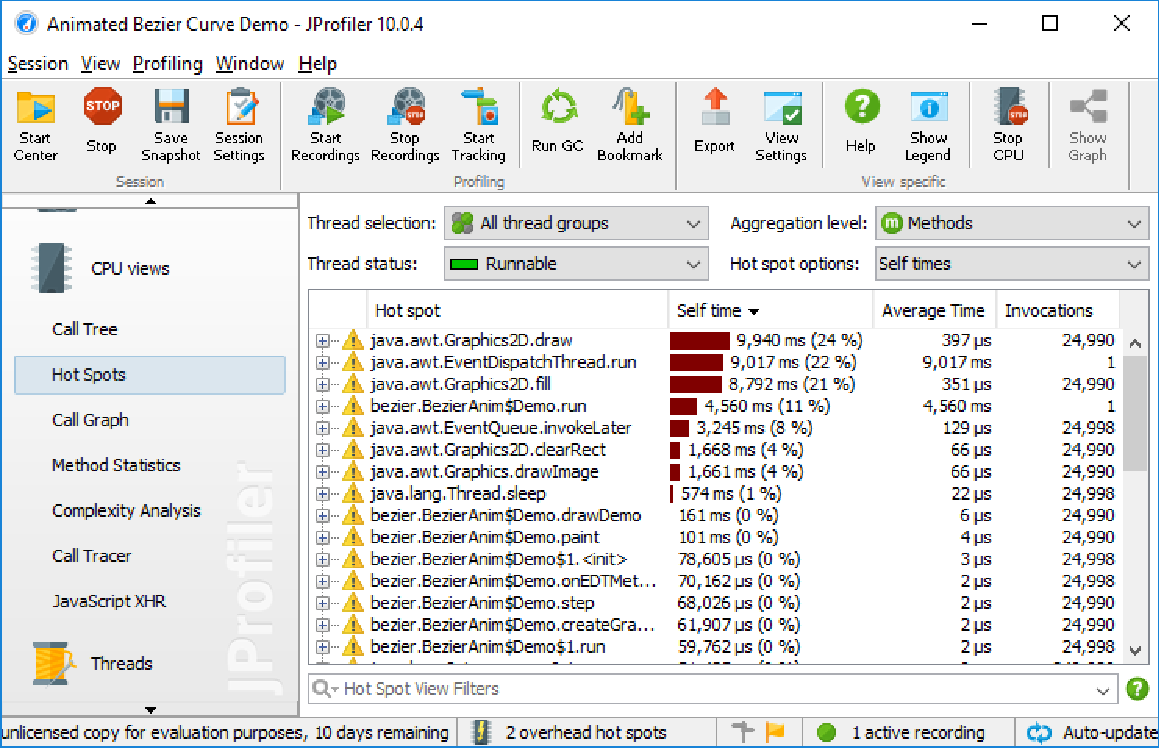
\includegraphics[width=0.8\textwidth]{invocations.pdf}}
\end{frame}

\lecturenotes
Профилировщик измеряет время, затраченное на выполнение каждого отдельного вызова метода. Таким образом, можно установить критические методы. Так же профилировщик может собирать дополнительную информацию, такую как дерево вызовов, состояние памяти, загруженность процессора. На изображении пример работы профайлера Jprofiler в режиме отображения "горячих мест".

\begin{frame} \frametitle{Количество вызовов каждого метода}
	\begin{block}{}
		Профилировщик может \alert{считать количество вызов} каждого метода. Данный функционал позволяет оптимизировать глубину дерева вызовов и уменьшить нагрузку
	\end{block}
	\centerline{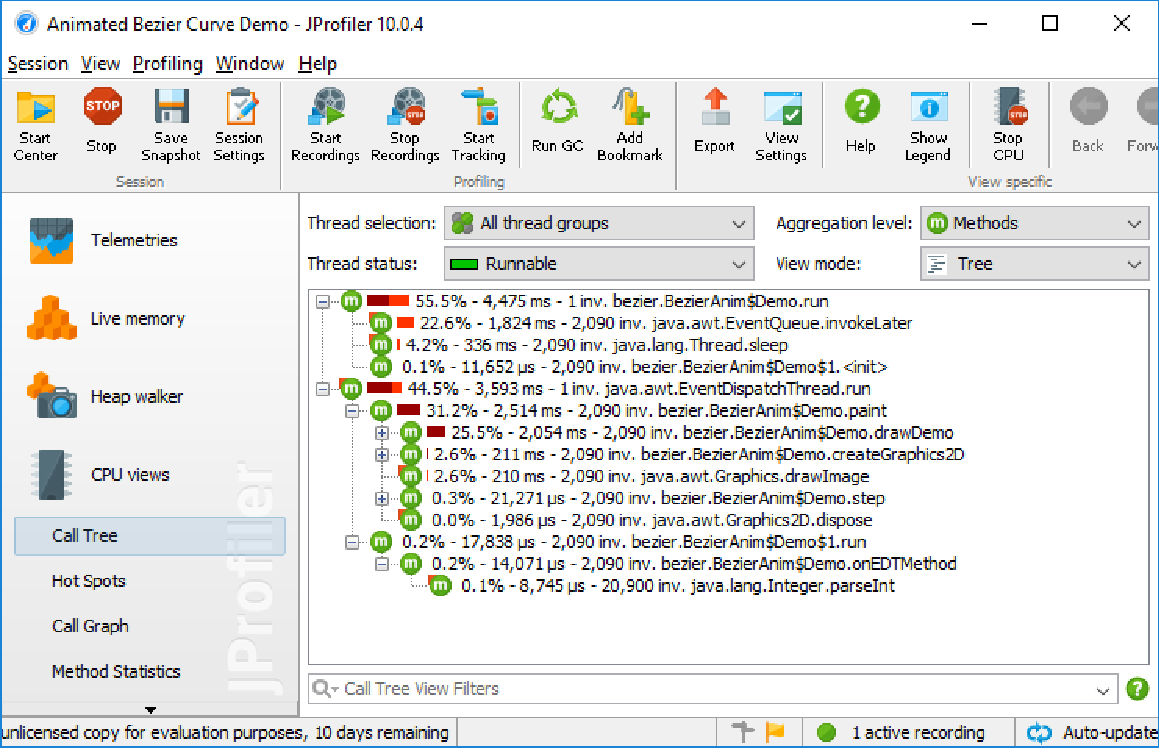
\includegraphics[width=0.8\textwidth]{calltree.pdf}}
\end{frame}

\lecturenotes
Профилировщик показывает сколько раз был вызван каждый метод. Обычно у профилировщика имеется функционал разделения контекста вызовов. Например, он может считать количество вызов в контексте всего жизненного цикла приложения или в контексте одного запроса. На изображении пример работы профайлера Jprofiler в режиме отображения дерева вызовов.

\begin{frame} \frametitle{Выделение памяти и сборка мусора}
	\begin{block}{}
		Профилировщик позволяет \alert{отслеживать изменения в~памяти}. Профилировщик позволяет видеть когда и в каком методе была выделена или освобождена память
	\end{block}
	\centerline{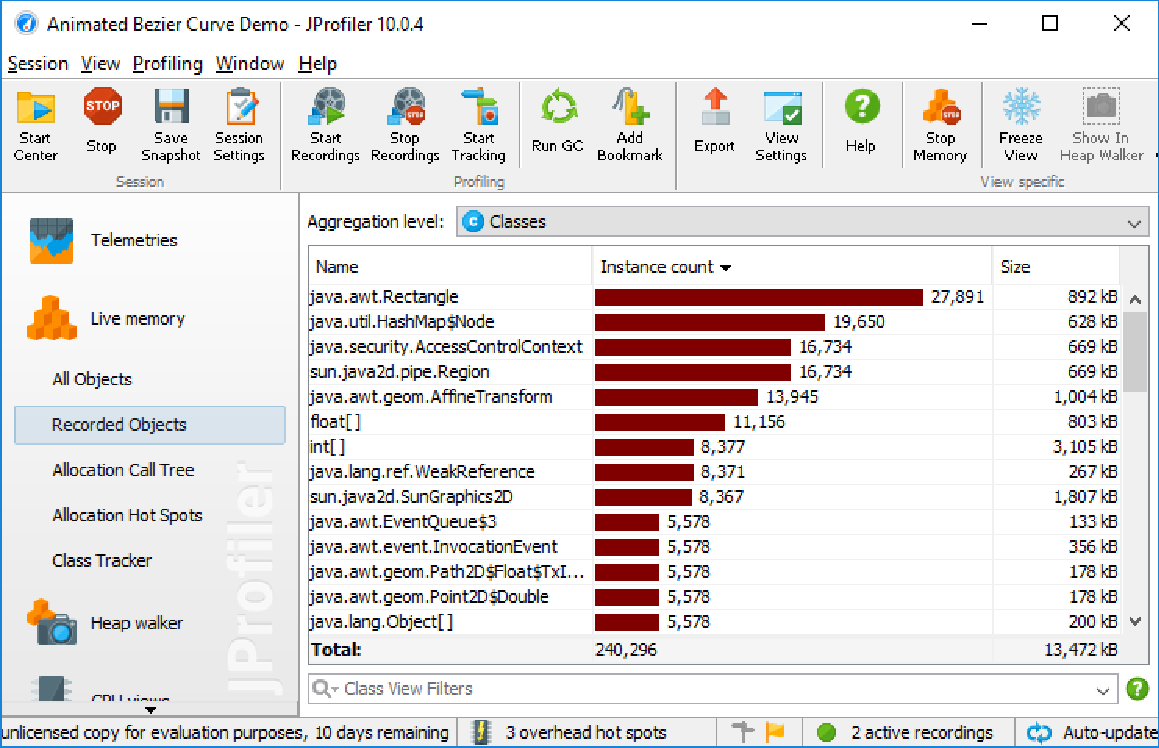
\includegraphics[width=0.8\textwidth]{memory.pdf}}
\end{frame}

\lecturenotes
Профилировщики обычно не включают по-умолчанию функционал профилирования памяти, т.к. это очень трудоёмкая процедура. Данная процедура позволяет увидеть все выделения и освобождения памяти. Обычно помечаются красным не освобождённые выделения, что позволяет быстро устранить утечку. На изображении пример работы профайлера Jprofiler в режиме отслеживания изменений в памяти.

\begin{frame} \frametitle{Время выполнения и количество WEB запросов}
	\begin{block}{}
		Профилировщики позволяют \alert{собирать информацию о Web--запросах}
	\end{block}
	\centerline{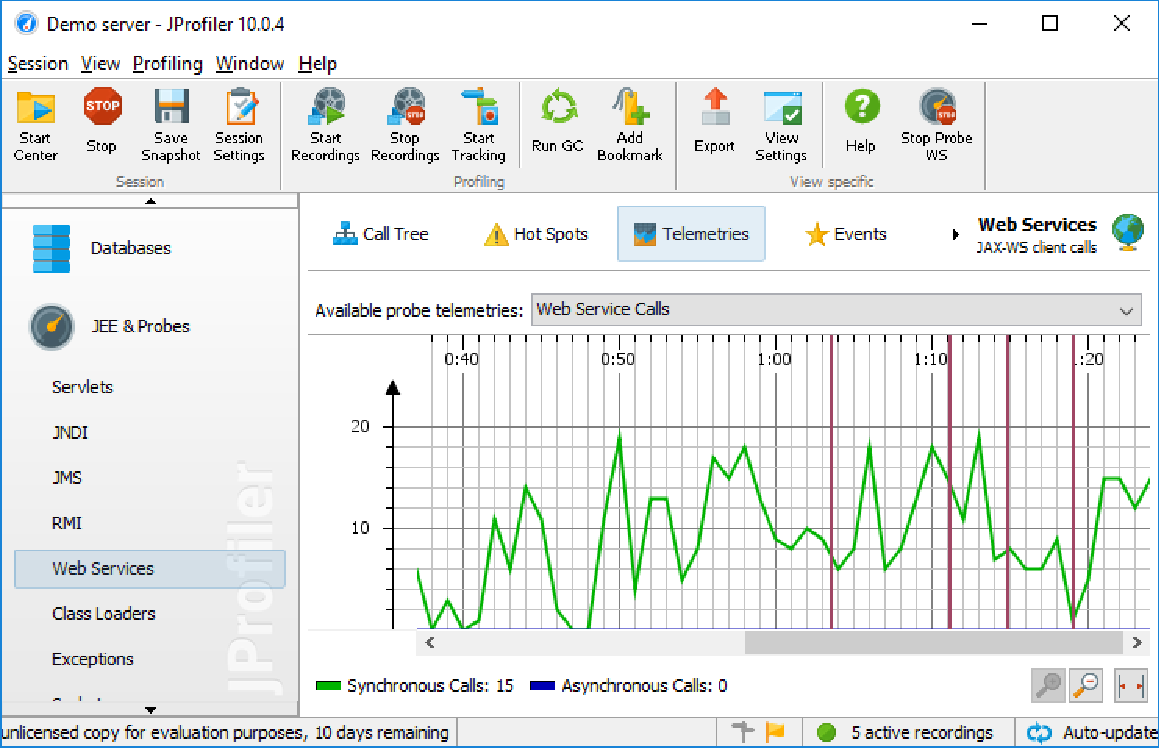
\includegraphics[width=0.8\textwidth]{webservices.pdf}}
\end{frame}
\lecturenotes
Профилирование веб-страниц позволяет найти критичные места в процессе загрузки страницы или REST-запроса. Обычно в итоге процедуры убирают дублирующие запросы, тяжёлые данные перемещают в кэш, а критичные тяжёлые запросы делают асинхронными. На изображении пример работы профайлера Jprofiler в режиме отображения интенсивности web-запросов.

\begin{frame} \frametitle{Время выполнения и количество WEB запросов}
	\centerline{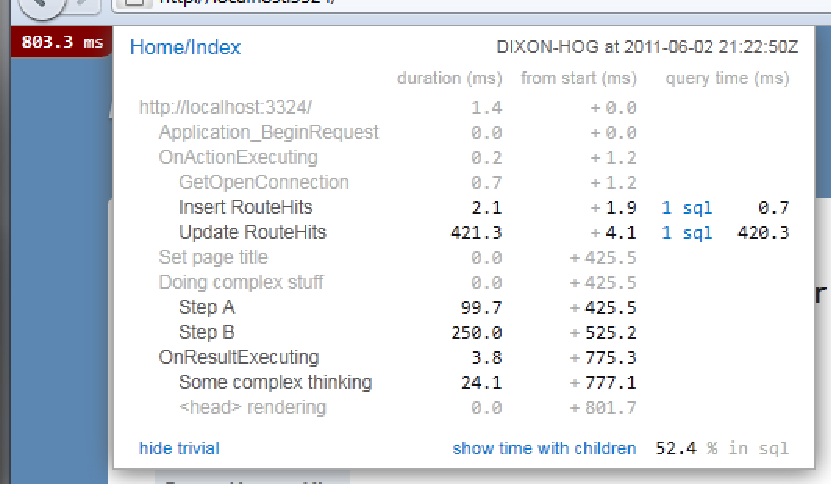
\includegraphics[width=0.8\textwidth]{miniprofiler1.pdf}}
\end{frame}
\lecturenotes
Профилировщики позволяют отслеживать web-запросы. Можно видеть интенсивность запросов и время их выполнения. На изображении пример вывода профилировщика MiniProfiler для .NET. Данный профилировщик высокоуровневый и может использоваться на тестовых стендах постоянно. Для тестировщиков и разработчиков данный профилирощик может сообщать об узких местах в отрисовке страницы, о дубликатах sql-запросов, о долгих sql-запросах.


\begin{frame} \frametitle{Время выполнения и количество WEB запросов}
	\centerline{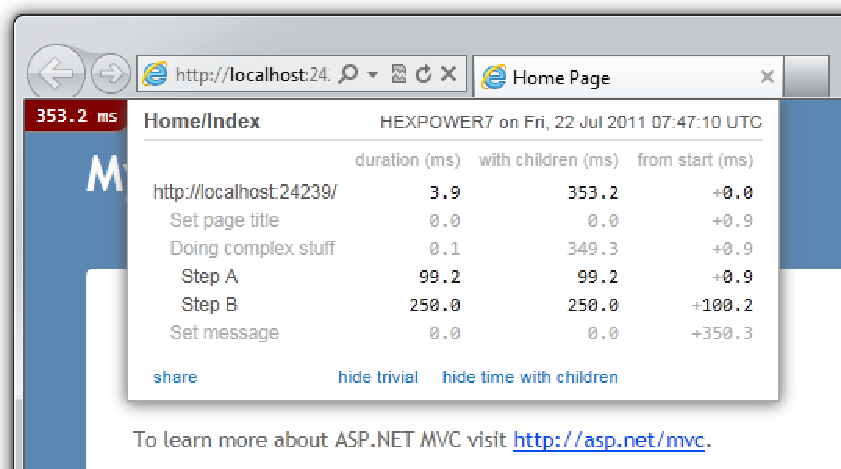
\includegraphics[width=0.8\textwidth]{miniprofiler2.pdf}}
\end{frame}
\lecturenotes
Данный профилировщик является высокоуровневым. Для отслеживания времени выполнения блоков кода их необходимо обернуть в using. Время выполнения и количество sql запросов отслеживается по-умолчанию. Miniprofiler часто используется на тестовых стендах совместно с отделом тестирования. При обнаружении проблем профилировщик показывает красным цветом в углу окна информацию об этих проблемах. Тестировщик копирует вывод профилировщика и сообщает о проблеме разработчикам. Таким образом получается ещё на этапе тестирования устранить множетво проблем с производительностью.


\begin{frame} \frametitle{Время выполнения и количество SQL запросов}
	\begin{block}{}
		Многие профилировщики позволяют \alert{собирать информацию о SQL--запросах}. Собираются такие данные как:
	\end{block}

	\begin{itemize}
	\item Количество запросов в контексте
	\item Дубликаты запросов
	\item Время затраченное на запрос/ответ к sql--серверу
	\item Количество передаваемой информации
	\end{itemize}

	\begin{block}{}
		В случае использования ORM так же может отслеживаться время, затраченное на построение запроса
	\end{block}
\end{frame}
\lecturenotes
Профилировщик позволяет собрать информацию о работе приложения с sql-сервером. Обычный профилировщик позволяет увидеть количество запросов, количество переданной и полученной информации, дублирующиеся запросы. Если профилировщик поддерживает использующуюся в коде приложения ORM, то его функционал значительно расширяется. Можно увидеть конкретные строки кода где запрос дублируется, оптимизировать время построения запроса. Например если запрос вызывается без изменения входных данных, то его можно сохранить в скомпилированном виде. В таком случае при следующем обращении к БД системе ORM не потребуется заново компилировать запрос.

\begin{frame} \frametitle{Время выполнения и количество SQL запросов}
	\centerline{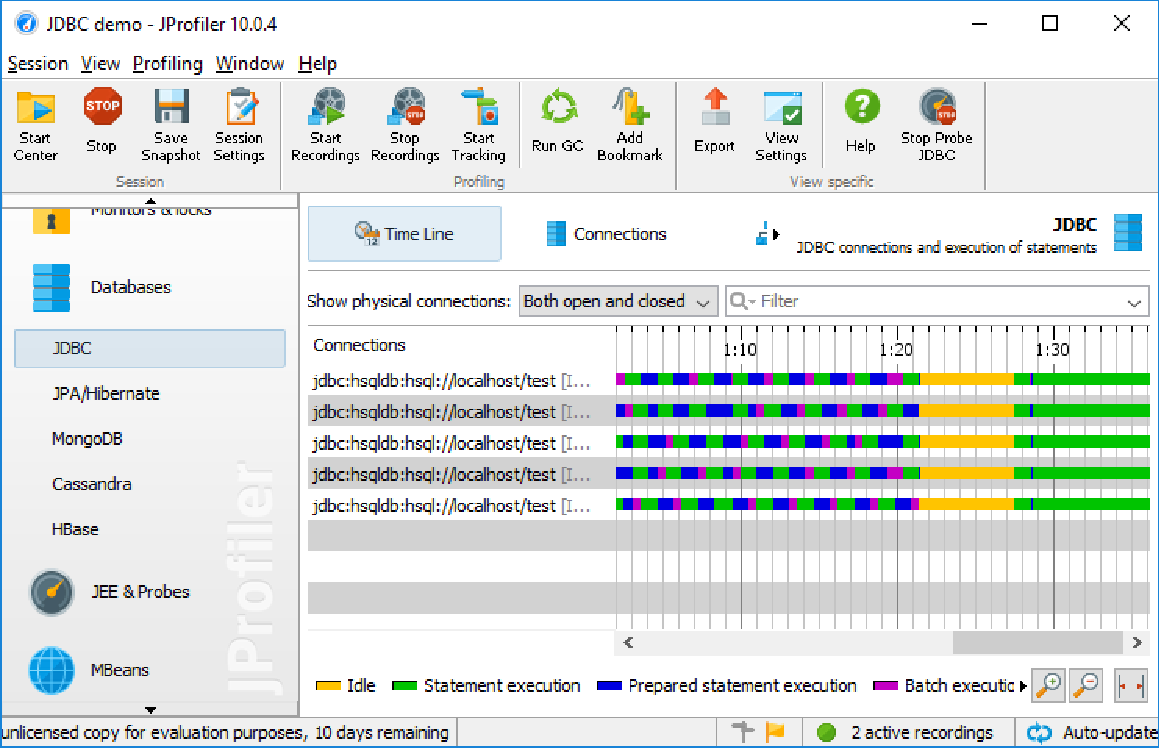
\includegraphics[width=0.8\textwidth]{database.pdf}}
\end{frame}
\lecturenotes
На изображении пример вывода профилировщика JProfiler в режиме анализа sql-запросов.

\section{Область применения процедуры профилирования~кода}

\begin{frame} \frametitle{Область применения процедуры профилирования кода}
	\begin{block}{}
		Процедура профилирования кода может применяться в любом программном продукте. Профилировщики разделяются на две основные группы:
	\end{block}
	
	\begin{itemize}
		\item Высокоуровневые
		\item Низкоуровневые
	\end{itemize}

	\begin{block}{}
		Низкоуровневые профилировщики \alert{крайне медленные} и обычно используются как <<средство последней надежды>>.
	\end{block}
\end{frame}

\lecturenotes
Профилировщики могут применяться в любом программном продукте. Выделяют две группы профилировщков: высокоуровневые и низкоуровневые. Высокоуровневые профилировщики отслеживают производительность приложения в целом (текущий уровень использования памяти, процессора, сети и т.д.) и, возможно, производительность ключевых блоков кода. Для отслеживания производительности ключевых блоков требуется незначительное изменение исходного кода (необходимо пометить ключевые методы или блоки). Высокоуровневые профилировщики позволяют получить доступ к логам и ошибкам приложения. Данные "пометки" можно не убирать в релизной версии приложения, т.к. профилировщик по-умолчанию настроен автоматически отключаеться когда выбрана конфигурация release.
Низкоуровневые профилировщики крайне медленные и обычно используются только в крайних случаях. Профилируются каждая строка кода, выделения памяти, сборка мусора.

\begin{frame} \frametitle{Область применения процедуры профилирования кода}
	\begin{block}{}
		По области применения выделяют три группы профилировщиков:
	\end{block}
	
	\begin{itemize}
		\item Профилирование методов или строк
		\item Трассировщики транзакций
		\item Профилирование производительности приложений (APM)
	\end{itemize}
\end{frame}
\lecturenotes
Профилирование методов или строк относится к низкоуровневым профилировщикам. Трассировщики транзакций позволяют отслеживать web и sql запросы. Профилирование производительности приложений позволяет увидеть информацию об используемых приложением ресурсами без доступа к исходному коду. Обычно применяется на серверах для выявляния тяжёлых приложений.

\section{Анализ профиля и техники оптимизации,~основанные на нём}
\begin{frame} \frametitle{Анализ профиля и техники оптимизации, основанные на нём}
	\begin{block}{}
		Первым шагом устраняются все <<простые>> ошибки:
	\end{block}
	
	\begin{itemize}
		\item Устранение дублирующихся вызовов и запросов
		\item Кэширование часто используемых данных
		\item Кэширование частых запросов к БД
	\end{itemize}
\end{frame}
\lecturenotes
На первом этапе оптимизации устраняются простые ошибки производительности. Обычно это дубликаты запросов в бд или во внешние сервисы, частое использование одинаковых данных. Самый очевидный вид оптимизации - оптимизация циклов. Циклы не должны содержать каких-либо внешних запросов. Необходимо перед выполнением цикла предзагрузить все необходимые даные и в теле цикла оперировать ими.

\begin{frame} \frametitle{Анализ профиля и техники оптимизации, основанные на нём}
	\begin{block}{}
		После нахождения критической части кода применяют следующие техники оптимизации:
	\end{block}
	
	\begin{itemize}
		\item Инициализация объектов данных
		\item Оптимизация арифметических операций
		\item Оптимизация циклов
		\item Выделение инвариантных фрагментов кода
	\end{itemize}
\end{frame}
\lecturenotes
1. Инициализация объектов данными. Объекты с необходимыми данными лучше всего инициализировать перед выполнением действий с ними, а не в самом процессе. Таким образом получается что все необходимые данные загружаются за один запрос и в процессе выполнения метода дополнительных запросов данных не будет.
На старых или медленных устройствах сократить процессорное время инициализацией массивов прямым присваиванием. Использование цикла, скорее всего, будет менее эффективным.
2. Оптимизация арифметических операций
Все константные операции следует помечать директивой const. Таким образом операция будет выполнена ещё на этапе компиляции и в итоговом коде она будет представлена в виде числа.
Так же следует заметить, что в большинстве архитектур быстрыми операциями являются сложение и вычитание. Затем идёт умножение, а за ним деление. Например выражение x / a, где а - константа для аргументов с плавающей точкой производится быстрее в виде x * b, где b = 1 / a - константа, вычисляемая на этапе компиляции. При большом количестве операций деления замена деления на умножение может дать существенный прирост производительности даже на мощных системах.
3. Оптимизация циклов
На современных машинах получить прирост производительности заменой одного типа цикла на другой практически невозможно. В современном мире оптимизировать циклы можно путём инициализации необходимых данных перед циклом см. пункт 1.

Так же необходимо минимизировать количество операций в цикле. Например если часть арифметического выражения статична, то можно вынести её в переменную, объявленную перед циклом. Таким образом можно сократить количество арифметических операций.
Данная операция называется выделением инфариантных фрагментов кода~\cite{Optimization}.

Важно:
Выполнение внешних запросов в цикле неприемлимо. Лучшая оптимизация цикла - избавление от цикла.

\section{Назначение процедуры статического анализа кода и её область применения}

\begin{frame} \frametitle{Назначение процедуры статического анализа кода}
	\begin{block}{}
		Статический анализ кода "--- это процесс выявления ошибок и недочетов в исходном коде программ. Статический анализ можно рассматривать как автоматизированный процесс обзора кода.
	\end{block}
\end{frame}
\lecturenotes
Статический анализ позволяет выявить ошибки в программе до компиляции исходного кода. Статические анализаторы могут быть встроенны в IDE или запускаться отдельно. Современные статические анализаторы позволяют анализировать код всего проекта "на лету" и давать советы по его оптимизации.

\begin{frame} \frametitle{Задачи процедуры статического анализа кода}
	\begin{block}{}
		Задачи, решаемые программами статического анализа кода можно разделить на 3 категории:
	\end{block}
	
	\begin{itemize}
		\item Выявление ошибок в программах
		\item Рекомендации по оформлению кода
		\item Подсчет метрик
	\end{itemize}

	\begin{block}{}
		Метрика программного обеспечения "--- это~мера,~позволяющая получить численное значение некоторого свойства программного обеспечения или его спецификаций
	\end{block}
	
\end{frame}
\lecturenotes
Современные статические анализаторы помогают быстро устранить ошибки в программах. Например Java Lint не даст скомпилировать программу в случае ошибки в синтаксисе кода. Практически все статические анализаторы поддерживают функционал стилистического анализа кода. В настройках анализатора указывается стилевой файл, содержащий принятый стиль оформления кода. В случае несоответсвия стилей, проблемный участок кода подсвечивается. Многие анализаторы помогают оптимизировать код непосредственно в процессе его написания. Для этого высчитываются метрики различных свойств ПО. Самый простой пример метрики - нахождение одинаковых фрагментов кода~\cite{StaticAnalisysMain}.

\begin{frame} \frametitle{Задачи процедуры статического анализа кода}
	\begin{block}{}
		Статический анализ часто используют как метод контроля и обучения новых сотрудников, еще недостаточно знакомых с правилами программирования в компании
	\end{block}
	\begin{block}{}
		Статический анализатор может быть установлен на сервер непрерывной интеграции. Специальные плагины могут отвергать коммиты при обнаружении в них проблем
	\end{block}
\end{frame}
\lecturenotes
Большинство компаний используют статические анализаторы для контроля и обучения новых сотрудников. Статический анализатор даёт новому сотрдунику подсказки по стилю оформления кода. Так же, часто стилевой анализатор устанавливается на сервер непрерывной интеграции и отвергает push в репозиторий при несоответствии кода заданному стилю.

\begin{frame} \frametitle{Задачи процедуры статического анализа кода}
	\centerline{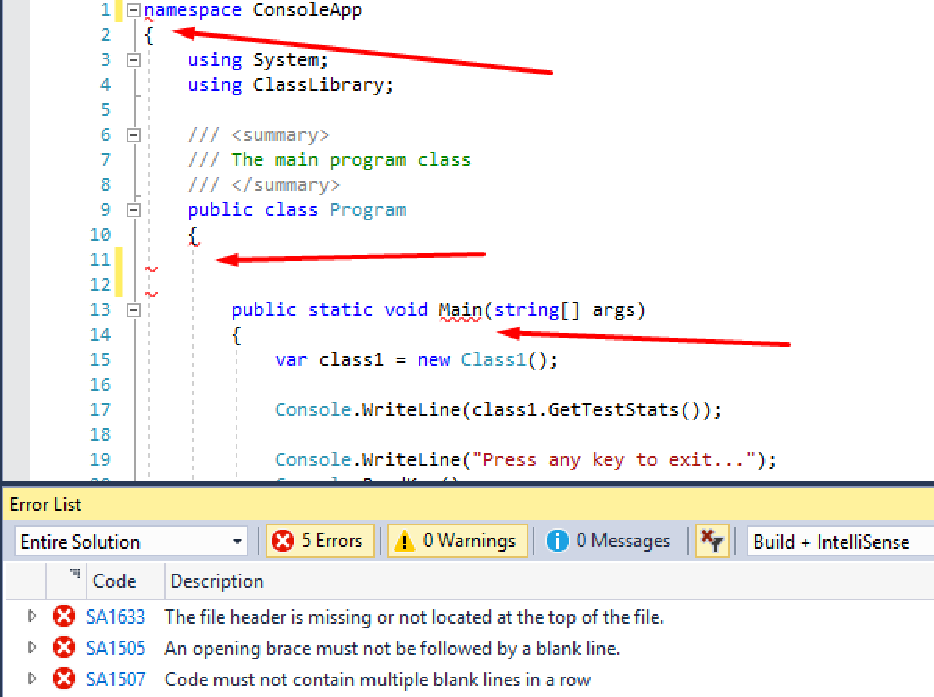
\includegraphics[width=0.8\textwidth]{stylecop.pdf}}
\end{frame}
\lecturenotes
На слайде показан вывод самого популярного стилистического анализатора для C\texttt{\#} - StyleCop. Обнаружены грубые ошибки в оформлении кода.

\section{Возможности существующих статических анализаторов}
\begin{frame} \frametitle{Возможности существующих статических анализаторов}
	\begin{block}{}
		Современные статические анализаторы позволяют проверять следующие параметры кода:
	\end{block}
	\begin{itemize}
		\item Корректность
		\item Удобство использования
		\item Безопасность
		\item Производительность
		\item Доступность
		\item i18n "--- интернационализация
	\end{itemize}
\end{frame}
\lecturenotes
Возможности статических анализаторов будем рассматривать на примере Android Lint~\cite{AndroidLint}. Android Lint является мощным и быстрым инструментом анализа кода. Данный анализатор умеет проверять такие аспекты как:
1. Корректность
Анализатор подсказывает явные синтаксические и логические ошибки.
2. Удобство использования
Анализатор помогает выделить фрагменты кода в методы. Анализатор может быть настроен на обязательное наличие комментария к методам.
3. Безопасность
Анализатор следит за обработкой checked исключений, выводит предупреждения об использовании неинициализированных объектов.
4. Производительность
Анализатор может давать советы по оптимизации кода. В частности это касается оптимизации циклов.
5. Доступность
Анализатор даёт советы по ограничении доступа к классам и методам. По умолчанию анализаторы настроены на максимальную инкапсуляцию классов и методов. Если метод используется только внутри класса, анализатор обязательно укажет, что необходимо использовать модификатор доступа private.
6. i18n - интернационализация
Подробности на следующем слайде.
Полный чек-лист проверок Android Lint доступен по ссылке~\cite{LintChecks}.

\begin{frame} \frametitle{i18n - интернационализация}
	\begin{block}{}
		\alert{Важно}: интернационализация != локализация
	\end{block}
	\begin{itemize}
		\item Избежание зависимости кода от значений строк пользователя
		\item Поддержка разметкой отображения интерфейса справа-налево
		\item Отображение нелатинских символов в разных локализациях
		\item Внесение предопределённых локализированных данных
		\item Выделение локализированных данных из кода
	\end{itemize}
\end{frame}
\lecturenotes
Важно: интернационализация - это не локализация.
Интернационализация кода позволяет легко локализовать продукт для целевых пользователей. i18n 18 - это число букв между 'i' and 'n' в слове internationalization.
Анализатор позволяет найти проблемы с интернационализацией. Например:
1. Избежание зависимости кода от значений строк пользователя.
Код не должен опираться на пользовательский ввод. Валидация пользовательского ввода должна быть независимой от локализации.
2. Проверка разметки на поддержку отображения интерфейса справа-налево.
Актуально, если продукт планируется выводить на арабский рынок.
3. Проверка возможности отображения нелатинских символов в разных локализациях.
Некоторые символы неподдерживаются на устройствах, где отстутствует локализация, из которой берётся символ. В крайнем случае можно использовать изображение требуемого символа.
4. Внесение предопределённых локализированных данных или черт, взятых из предпочтений пользователя. Например: форматы дат и времени, местные календари, числовые форматы и числовые системы, отбор и представление списков, обращение с личными именами и форм обращения.
5. Выделение локализованных данных из кода, таким образом, чтобы локализированные варианты можно было загрузить позже или выбрать, основываясь на предпочтениях пользователя. В android это файлы strings.xml, расположенные в папках values-** с соответстующим кодом локализации~\cite{i18n}.

\section{Роль статического анализа в промышленной разработке}
\begin{frame} \frametitle{Роль статического анализа в промышленной разработке}
	\begin{block}{}
		Статический анализатор позволяет значительно сэкономить ресурсы компании
	\end{block}
	\begin{itemize}
		\item Выявление большого числа ошибок на стадии разработки
		\item Быстрая интеграция новых членов команды
		\item Поддержание <<чистоты>> кода
		\item Поддержание корпоративного стиля кода
	\end{itemize}
\end{frame}
\lecturenotes
Современная компания-разработчик ПО обязана иметь инструменты для статического анализа. Анализатор позволяет отсеять простые логические ошибки и ошибки безопасноти использования кода на стадии разработки. Опыт показывает что таких ошибок может быть много. Таким образом значительно уменьшается время тестирования продукта.
Как говорилось ранее, статический анализатор значительно ускоряет процесс вхождения новичков в работу.
Статический анализатор обеспечивает чистый код. В чистом коде разработчики работают гораздо продуктивнее. Таким образом снижаются затраты на разработку. Так же обеспечивается единообразие кода путём соответсвия корпоративному стилю.
В совокупности, правильно настроенный статический анализатор экономит массу ресурсов компании~\cite{StaticAnalisys}.

\begin{thebibliography}{99}
	\bibitem{Profiling} \href{https://stackify.com/what-is-code-profiling/}{What is code profiling?}
	\bibitem{Optimization} \href{http://www.azillionmonkeys.com/qed/optimize.html}{Programming Optimization}
	\bibitem{StaticAnalisysMain} \href{https://www.viva64.com/en/t/0046/}{Static code analysis}
	\bibitem{i18n} \href{https://www.w3.org/International/questions/qa-i18n.ru}{Локализация по сравнению с интернационализацией}
	\bibitem{AndroidLint} \href{https://developer.android.com/studio/write/lint.html}{Improve Your Code with Lint}
	\bibitem{LintChecks} \href{http://tools.android.com/tips/lint-checks}{Android Lint Checks}
	\bibitem{StaticAnalisys} \href{https://habrahabr.ru/company/pvs-studio/blog/331724/}{Статический анализ как часть процесса разработки Unreal Engine}
\end{thebibliography}

\end{document}

%%% Local Variables: 
%%% mode: TeX-pdf
%%% TeX-master: t
%%% End: 
